Consider a shear testing device consisting of two plates with a small piece of material between them. We apply a force $F$ continuously on the upper plate. The shear stress $\tau$ is defined as the amount of force per unit area,
\begin{equation}
  \tau = \frac{F}{A}
\end{equation}
where A is the area of the plate in contact with the fluid.

\begin{figure}[h] \label{fig:shear-testing}
  \centering
  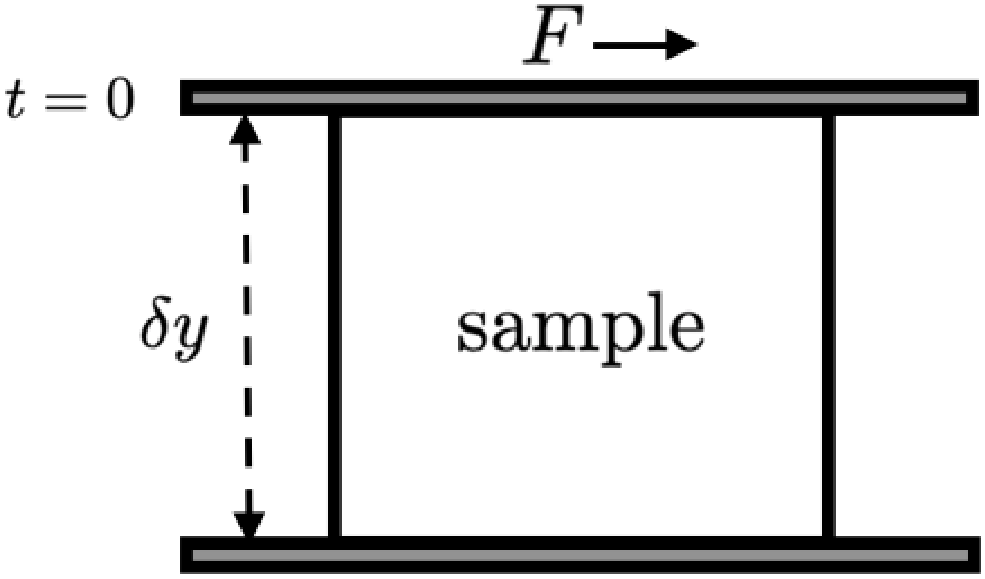
\includegraphics[width=6cm]{fig/shear-testing.png}
  \caption{A shear testing device (depicted in 2D).}
\end{figure}

%   ----    ----    SHEAR IN SOLIDS    ----    ----    %

\subsection{Shear in solids}

Consider the sample in our shear testing device is a solid, \figref{fig:shear-solids} shows the deformation after time $t'$. For any given shear $\tau$, the shear deformation is finite in solids. We can define a new quantity, shear strain $\lambda$, to measure this deformation:

\begin{equation}
  \lambda = \frac{ \Delta x }{ \delta y }
\end{equation}

\begin{figure} \label{fig:shear-solids}
  \centering
  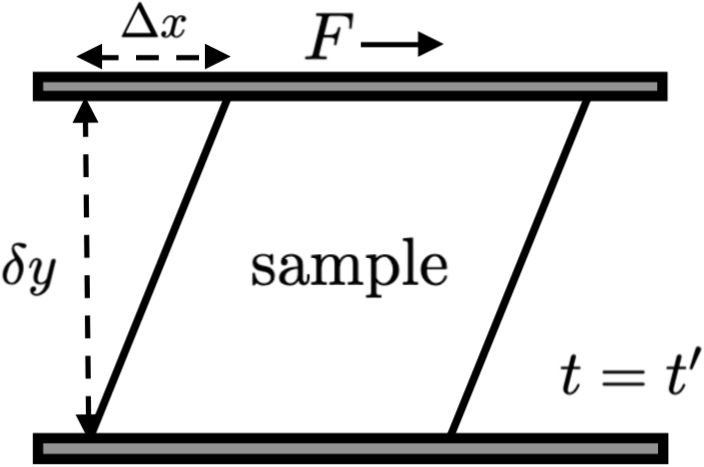
\includegraphics[width=5.5cm]{fig/shear-solid.png}
  \caption{Shear deformation at time $t>0$ for a solid.}
\end{figure}

We can derive the relationship between shear stress and strain experimentally. In fact, it turns out they are related linearly. We call the constant of proportionality the \textit{shear modulus}, $G$, and it is dependent on the material.

\begin{equation}\label{eq:shear-in-solids}
  \tau = G \lambda
\end{equation}

%   ----    ----    SHEAR IN FLUIDS    ----    ----    %

\subsection{Shear in fluids}

In comparison to the behaviour in solids, when a continuous shear stress is applied to a fluid it continues to deform indefinitely, assuming there are no counteracting forces. We can define what a fluid is according to this behaviour.

\begin{definition}
  A \textbf{fluid} is any material that is unable to prevent the deformation caused by shear stress.
\end{definition}

\begin{figure}[h] \label{fig:shear-fluid}
  \centering
  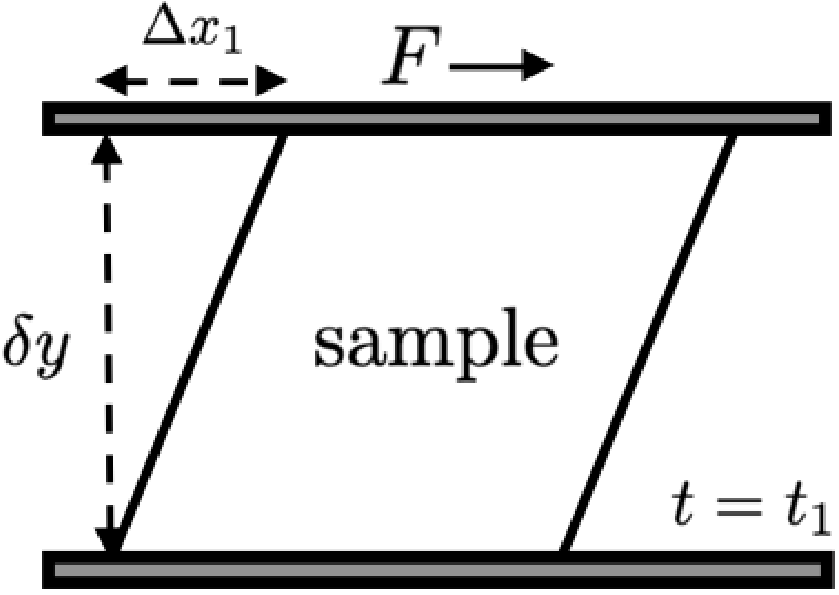
\includegraphics[width=5.05cm]{fig/shear-fluid-t1.png}
  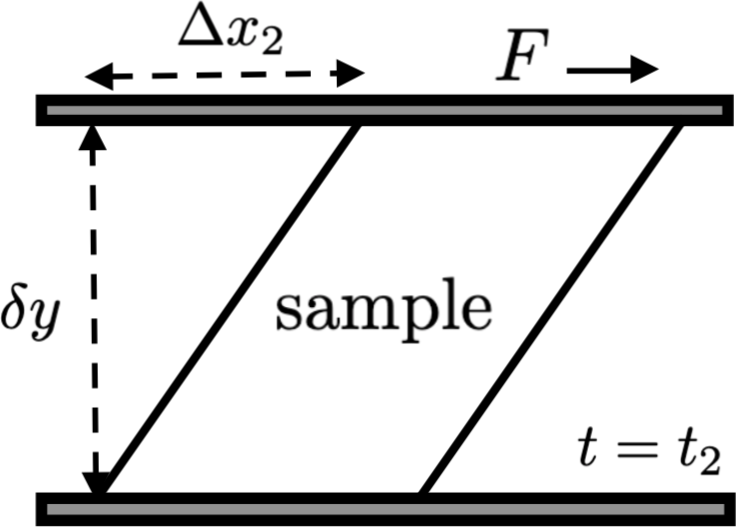
\includegraphics[width=4.95cm]{fig/shear-fluid-t2.png}
  \caption{Shear deformation for $t>0$ in a fluid.}
\end{figure}

Experimentally, we find that

\begin{equation}
  \tau \propto \frac{ d \lambda }{ d t }.
\end{equation}

In particularly, for Newtonian fluids we find that this relationship is linear. We call the constant of proportionality the \textit{absolute} or \textit{dynamic viscosity}, $\mu$.

\begin{equation} \label{eq:shear-stress-strain-in-liquids}
  \tau = \mu \frac{ d \lambda }{ d t }
\end{equation}

\begin{proposition}
  For a fluid with velocity $\vec{u} = (u,v,w)$, where $u$ is the velocity component in the direction of the shear stress,

  \begin{equation*}
    \tau = \mu \frac{ d u }{ d y }.
  \end{equation*}
\end{proposition}

\begin{proof}
  Consider our shear testing device as $\delta y \rightarrow 0$. Then,
  \begin{equation*}
    \tau = \lim_{\delta y \rightarrow 0} \frac{ d \lambda }{ dt } = \lim_{\delta y \rightarrow 0} \frac{ d }{ dt } \frac{ \Delta x }{ \delta y }
  \end{equation*}
  since we know that $\lambda = \Delta x / \delta y$
\end{proof}
